\documentclass[a4paper,12pt]{article}

\usepackage[utf8]{inputenc}
\usepackage[spanish]{babel}
\usepackage{amsmath, amssymb}
\usepackage{graphicx}
\usepackage{float}
\usepackage{booktabs}
\usepackage{xcolor}
\usepackage{listings}
\usepackage{caption}
\usepackage{fancyhdr}
\usepackage{hyperref}
\usepackage{tikz}

\hypersetup{
    colorlinks=true,
    linkcolor=blue,
    urlcolor=blue,
    pdftitle={Práctica 2 - Zebboard},
}

% === Definición de colores similares a Vivado ===
\definecolor{vivadoKeyword}{rgb}{0.6,0.0,0.6}
\definecolor{vivadoComment}{rgb}{0.0,0.5,0.0}
\definecolor{vivadoString}{rgb}{0.5,0.2,0.0}
\definecolor{vivadoBackground}{rgb}{0.97,0.97,0.97}

\lstdefinelanguage{VHDL}{
    morekeywords={library, use, entity, is, port, in, out, end, architecture, of, begin, signal, if, then, else, when, others, xor, and, or, not},
    sensitive=true,
    morecomment=[l]--,
    morestring=[b]",
}

\lstset{
    language=VHDL,
    backgroundcolor=\color{vivadoBackground},
    keywordstyle=\color{vivadoKeyword}\bfseries,
    commentstyle=\color{vivadoComment}\itshape,
    stringstyle=\color{vivadoString},
    basicstyle=\ttfamily\small,
    numbers=left,
    numberstyle=\tiny,
    numbersep=5pt,
    frame=single,
    breaklines=true,
    tabsize=2,
    captionpos=b
}

\title{Práctica N°2: Sumador de 3 bits usando pantalla OLED en placa ZedBoard}
\date{}

\begin{document}
\maketitle
\tableofcontents
\newpage

\section{Objetivos}

\subsection{Objetivo general}
Implementar en VHDL un \textbf{sumador de 3 bits} sobre la plataforma \textit{ZedBoard}, \textbf{reutilizando la base existente de la OLED} (SSD1306) con cambios mínimos al proyecto, de modo que los operandos \(\mathbf{A}\) y \(\mathbf{B}\) se ingresen por interruptores y el resultado \(\mathbf{A+B}\) se visualice en la pantalla OLED.

\subsection{Objetivos específicos}
\begin{enumerate}
    \item \textbf{Encapsular la aritmética:} diseñar e integrar un bloque \texttt{adder3} que sume dos vectores de 3 bits y entregue un resultado de 4 bits, evitando conflictos de librerías en el código legado.
    \item \textbf{Exposición de señales:} añadir puertos \texttt{a[2:0]} y \texttt{b[2:0]} en el nivel superior (\texttt{oled\_ctrl}) y enrutar estas señales hasta \texttt{oled\_ex}.
    \item \textbf{Actualización mínima del demo OLED:} modificar exclusivamente la rama de contenido en \texttt{oled\_ex} para construir y mostrar la cadena \texttt{"A=\_ B=\_ A+B=\_"} en formato hexadecimal (1 dígito por operando y 1 dígito para el resultado).
    \item \textbf{Soporte de caracteres:} verificar y, de ser necesario, añadir en \texttt{ascii\_rom} los glifos de \texttt{'+'} (0x2B) y \texttt{'='} (0x3D) sin alterar el resto de la ROM.
    \item \textbf{Asignación de pines:} mapear los bits de \texttt{a} y \texttt{b} a los \textit{switches} físicos de la ZedBoard mediante el archivo de restricciones, manteniendo intacta la lógica de inicialización y SPI.
    \item \textbf{Verificación funcional:} comprobar en hardware que para todos los casos \(A,B \in [0,7]\) la OLED muestre correctamente \(A\), \(B\) y \(A+B\) (0–14), incluyendo casos de “overflow” (por ejemplo \(7+7=14\)).
    \item \textbf{Criterios de éxito:} la visualización debe actualizarse sin \textit{glitches}, el proyecto debe sintetizar sin advertencias críticas y no deben introducirse modificaciones innecesarias fuera de los puntos descritos.
\end{enumerate}

\newpage

\section{Descripción del código}

Para esta práctica se \textbf{reutilizan exactamente los mismos archivos de inicialización y control SPI} de la práctica anterior (\,\texttt{oled\_init.vhd}, \texttt{spi\_ctrl.vhd}, \texttt{delay.vhd} y \texttt{ascii\_rom.vhd}\,), de forma que \textbf{no se tocan sus máquinas de estados ni sus temporizaciones}. El cambio es mínimo y se concentra en \textbf{tres puntos}: (1) en el \emph{top module} (\texttt{oled\_ctrl.vhd}) se exponen los puertos \texttt{a[2:0]} y \texttt{b[2:0]} para llevar los switches a la jerarquía; (2) se \textbf{crea} un bloque nuevo \texttt{adder3.vhd} encargado exclusivamente de la suma en 3+3 bits (aislando las librerías aritméticas); y (3) se \textbf{modifica} \texttt{oled\_ex.vhd} únicamente en la rama que arma el texto para la OLED, sustituyendo el mensaje de demo por la visualización de \texttt{A, B} y \texttt{A+B}. Este enfoque minimiza el riesgo de efectos colaterales y obliga a una separación clara de responsabilidades (inicialización, SPI, aritmética y presentación).

\subsection{Módulo 1: \texttt{adder3} (sumador 3+3 bits)}

\begin{lstlisting}[language=VHDL, caption={Bloque de suma aislado \texttt{adder3.vhd} (3+3 bits $\rightarrow$ 4 bits).}]
library IEEE;
use IEEE.STD_LOGIC_1164.ALL;
use IEEE.NUMERIC_STD.ALL;

entity adder3 is
  port (
    a    : in  std_logic_vector(2 downto 0);
    b    : in  std_logic_vector(2 downto 0);
    sum4 : out std_logic_vector(3 downto 0)   -- resultado 0..14
  );
end entity;

architecture rtl of adder3 is
begin
  -- Suma desambiguada dentro del bloque (solo numeric_std aquí)
  sum4 <= std_logic_vector( unsigned('0' & a) + unsigned('0' & b) );
end architecture;
\end{lstlisting}

\paragraph{¿Qué hace y por qué así?}
\begin{itemize}
  \item \textbf{Entradas y salida}. Recibe dos operandos de 3 bits (\(A\) y \(B\)) y entrega un resultado de 4 bits \( \texttt{sum4} \in [0,14]\). El bit extra cubre el posible acarreo en \(7+7\).
  \item \textbf{Extensión de tamaño}. La expresión \texttt{'0' \& a} (y análoga para \texttt{b}) antepone un cero para extender cada operando a 4 bits antes de sumar.
  \item \textbf{Aritmética tipada}. Se realiza el \emph{cast} a \texttt{unsigned} y se usa \texttt{numeric\_std}, lo que \textbf{evita ambigüedades de sobrecarga} del operador \texttt{+}. Luego se convierte el resultado a \texttt{std\_logic\_vector} para compatibilizar con el resto del diseño.
  \item \textbf{Encapsulación}. Al aislar la suma aquí, \textbf{no se modifican} los paquetes usados en archivos heredados (que emplean \texttt{std\_logic\_arith}/\texttt{std\_logic\_unsigned}). Así prevenimos conflictos sin refactorizar el legado.
  \item \textbf{Uso previsto}. Este bloque se instancia en \texttt{oled\_ex.vhd}, y su salida \texttt{sum4} se convierte a ASCII (hex) para mostrar \texttt{A}, \texttt{B} y \texttt{A+B} en la OLED.
\end{itemize}

\subsection{Módulo 2: \texttt{oled\_ex} (demo OLED + visualización de A, B y A+B)}

\begin{lstlisting}[language=VHDL, caption={\texttt{oled\_ex.vhd}: demo de OLED adaptado para mostrar A, B y A+B en la primera línea.}]
--
-- Written by Ryan Kim, Digilent Inc.
-- Modified by Michael Mattioli
--
-- Description: Demo for the OLED display. First displays the alphabet for ~4 seconds and then
-- clears the display, waits for a ~1 second and then displays "Hello world!".
--

library ieee;
use ieee.std_logic_1164.all;
use ieee.std_logic_arith.all;
use ieee.std_logic_unsigned.all;

entity oled_ex is
    port (  clk         : in std_logic; -- System clock
            rst         : in std_logic; -- Global synchronous reset
            en          : in std_logic; -- Block enable pin
            sdout       : out std_logic; -- SPI data out
            oled_sclk   : out std_logic; -- SPI clock
            oled_dc     : out std_logic; -- Data/Command controller
            fin         : out std_logic; -- Finish flag for block
            a    : in std_logic_vector(2 downto 0); -- 3 bits
            b     : in std_logic_vector(2 downto 0));  -- 3 bits
end oled_ex;

architecture behavioral of oled_ex is

    -- SPI controller
    component spi_ctrl
        port (  clk         : in std_logic;
                rst         : in std_logic;
                en          : in std_logic;
                sdata       : in std_logic_vector (7 downto 0);
                sdout       : out std_logic;
                oled_sclk   : out std_logic;
                fin         : out std_logic);
    end component;

    -- delay controller
    component delay
        port (  clk         : in std_logic;
                rst         : in std_logic;
                delay_ms    : in std_logic_vector (11 downto 0);
                delay_en    : in std_logic;
                delay_fin   : out std_logic);
    end component;

    -- character library, latency = 1
    component ascii_rom
        port (  clk    : in std_logic; -- System clock
                addr   : in std_logic_vector (10 downto 0); -- First 8 bits is the ASCII value of the character, the last 3 bits are the parts of the char
                dout   : out std_logic_vector (7 downto 0)); -- Data byte out
    end component;

    -- States for state machine
    type states is (Idle,
                    ClearDC,
                    SetPage,
                    PageNum,
                    LeftColumn1,
                    LeftColumn2,
                    SetDC,
                    Alphabet,
                    Wait1,
                    ClearScreen,
                    Wait2,
                    HelloWorldScreen,
                    UpdateScreen,
                    SendChar1,
                    SendChar2,
                    SendChar3,
                    SendChar4,
                    SendChar5,
                    SendChar6,
                    SendChar7,
                    SendChar8,
                    ReadMem,
                    ReadMem2,
                    Done,
                    Transition1,
                    Transition2,
                    Transition3,
                    Transition4,
                    Transition5);

    type oled_mem is array (0 to 3, 0 to 15) of std_logic_vector (7 downto 0);
    
    -- Variable that contains what the screen will be after the next UpdateScreen state
    signal current_screen : oled_mem;
    
    signal sum4 : std_logic_vector(3 downto 0);
    
    -- Convierte 0..15 a '0'..'9','A'..'F'
function nibble_to_ascii(n : std_logic_vector(3 downto 0))
  return std_logic_vector is
    begin
      case n is
        when "0000" => return x"30"; -- '0'
        when "0001" => return x"31";
        when "0010" => return x"32";
        when "0011" => return x"33";
        when "0100" => return x"34";
        when "0101" => return x"35";
        when "0110" => return x"36";
        when "0111" => return x"37";
        when "1000" => return x"38";
        when "1001" => return x"39";
        when "1010" => return x"41"; -- 'A'
        when "1011" => return x"42";
        when "1100" => return x"43";
        when "1101" => return x"44";
        when "1110" => return x"45";
        when others => return x"46"; -- 'F'
      end case;
    end function;

    -- Constant that contains the screen filled with the Alphabet and numbers
    constant alphabet_screen : oled_mem := ((x"41", x"42", x"43", x"44", x"45", x"46", x"47", x"48", x"49", x"4A", x"4B", x"4C", x"4D", x"4E", x"4F", x"50"),
    (x"51", x"52", x"53", x"54", x"55", x"56", x"57", x"58", x"59", x"5A", x"61", x"62", x"63", x"64", x"65", x"66"),
    (x"67", x"68", x"69", x"6A", x"6B", x"6C", x"6D", x"6E", x"6F", x"70", x"71", x"72", x"73", x"74", x"75", x"76"),
    (x"77", x"78", x"79", x"7A", x"30", x"31", x"32", x"33", x"34", x"35", x"36", x"37", x"38", x"39", x"7F", x"7F"));

    -- Constant that fills the screen with blank (spaces) entries
    constant clear_screen : oled_mem := (   (x"20", x"20", x"20", x"20", x"20", x"20", x"20", x"20", x"20", x"20", x"20", x"20", x"20", x"20", x"20", x"20"),
    (x"20", x"20", x"20", x"20", x"20", x"20", x"20", x"20", x"20", x"20", x"20", x"20", x"20", x"20", x"20", x"20"),
    (x"20", x"20", x"20", x"20", x"20", x"20", x"20", x"20", x"20", x"20", x"20", x"20", x"20", x"20", x"20", x"20"),
    (x"20", x"20", x"20", x"20", x"20", x"20", x"20", x"20", x"20", x"20", x"20", x"20", x"20", x"20", x"20", x"20"));

    -- Constant that holds "Hello world!"
    constant hello_world_screen : oled_mem := ( (x"48", x"65", x"6c", x"6c", x"6f", x"20", x"77", x"6f", x"72", x"6c", x"64", x"21", x"20", x"20", x"20", x"20"),
    (x"20", x"20", x"20", x"20", x"20", x"20", x"20", x"20", x"20", x"20", x"20", x"20", x"20", x"20", x"20", x"20"),
    (x"20", x"20", x"20", x"20", x"20", x"20", x"20", x"20", x"20", x"20", x"20", x"20", x"20", x"20", x"20", x"20"),
    (x"20", x"20", x"20", x"20", x"20", x"20", x"20", x"20", x"20", x"20", x"20", x"20", x"20", x"20", x"20", x"20"));

    -- Current overall state of the state machine
    signal current_state : states := Idle;

    -- State to go to after the SPI transmission is finished
    signal after_state : states;

    -- State to go to after the set page sequence
    signal after_page_state : states;

    -- State to go to after sending the character sequence
    signal after_char_state : states;

    -- State to go to after the UpdateScreen is finished
    signal after_update_state : states;

    -- Contains the value to be outputted to oled_dc
    signal temp_dc : std_logic := '0';

    -- Used in the Delay controller block
    signal temp_delay_ms : std_logic_vector (11 downto 0); -- Amount of ms to delay
    signal temp_delay_en : std_logic := '0'; -- Enable signal for the Delay block
    signal temp_delay_fin : std_logic; -- Finish signal for the Delay block

    -- Used in the SPI controller block
    signal temp_spi_en : std_logic := '0'; -- Enable signal for the SPI block
    signal temp_sdata : std_logic_vector (7 downto 0) := (others => '0'); -- Data to be sent out on SPI
    signal temp_spi_fin : std_logic; -- Finish signal for the SPI block

    signal temp_char : std_logic_vector (7 downto 0) := (others => '0'); -- Contains ASCII value for character
    signal temp_addr : std_logic_vector (10 downto 0) := (others => '0'); -- Contains address to byte needed in memory
    signal temp_dout : std_logic_vector (7 downto 0); -- Contains byte outputted from memory
    signal temp_page : std_logic_vector (1 downto 0) := (others => '0'); -- Current page
    signal temp_index : integer range 0 to 15 := 0; -- Current character on page

begin

    oled_dc <= temp_dc;

    -- "Example" finish flag only high when in done state
    fin <= '1' when current_state = Done else '0';

    -- Instantiate SPI controller
    spi_comp: spi_ctrl port map (   clk => clk,
                                    rst => rst,
                                    en => temp_spi_en,
                                    sdata => temp_sdata,
                                    sdout => sdout,
                                    oled_sclk => oled_sclk,
                                    fin => temp_spi_fin);

    -- Instantiate delay
    delay_comp: delay port map (clk => clk,
                                rst => rst,
                                delay_ms => temp_delay_ms,
                                delay_en => temp_delay_en,
                                delay_fin => temp_delay_fin);

    -- Instantiate ASCII character library
    char_lib_comp : ascii_rom port map (clk => clk,
                                        addr => temp_addr,
                                        dout => temp_dout);
                                        
    u_adder3 : entity work.adder3 port map (
                a    => a,
                b    => b,
                sum4 => sum4);

    process (clk)
    begin
        if rising_edge(clk) then
            case current_state is
                -- Idle until en pulled high than intialize Page to 0 and go to state alphabet afterwards
                when Idle =>
                    if en = '1' then
                        current_state <= ClearDC;
                        after_page_state <= Alphabet;
                        temp_page <= "00";
                    end if;
                -- Set current_screen to constant alphabet_screen and update the screen; go to state Wait1 afterwards
                when Alphabet =>
                    current_screen <= alphabet_screen;
                    current_state <= UpdateScreen;
                    after_update_state <= Wait1;
                -- Wait 4ms and go to ClearScreen
                when Wait1 =>
                    temp_delay_ms <= "111110100000"; -- 4000
                    after_state <= ClearScreen;
                    current_state <= Transition3; -- Transition3 = delay transition states
                -- Set current_screen to constant clear_screen and update the screen; go to state Wait2 afterwards
                when ClearScreen =>
                    current_screen <= clear_screen;
                    after_update_state <= Wait2;
                    current_state <= UpdateScreen;
                -- Wait 1ms and go to HelloWorldScreen
                when Wait2 =>
                    temp_delay_ms <= "001111101000"; -- 1000
                    after_state <= HelloWorldScreen;
                    current_state <= Transition3; -- Transition3 = delay transition states
                -- Set currentScreen to constant hello_world_screen and update the screen; go to state Done afterwards
                when HelloWorldScreen =>
                    -- Limpiar la pantalla base
                    current_screen <= clear_screen;
                
                    -- Línea 0: "A=H B=H A+B=H" (H = digito HEX)
                    current_screen(0, 0)  <= x"41";                    -- 'A'
                    current_screen(0, 1)  <= x"3D";                    -- '='
                    current_screen(0, 2)  <= nibble_to_ascii('0' & a); -- A (hex)
                
                    current_screen(0, 3)  <= x"20";                    -- espacio
                    current_screen(0, 4)  <= x"42";                    -- 'B'
                    current_screen(0, 5)  <= x"3D";                    -- '='
                    current_screen(0, 6)  <= nibble_to_ascii('0' & b); -- B (hex)
                
                    current_screen(0, 7)  <= x"20";                    -- espacio
                    current_screen(0, 8)  <= x"41";                    -- 'A'
                    current_screen(0, 9)  <= x"2B";                    -- '+'
                    current_screen(0,10)  <= x"42";                    -- 'B'
                    current_screen(0,11)  <= x"3D";                    -- '='
                    current_screen(0,12)  <= nibble_to_ascii(sum4);    -- A+B (hex)
                
                    -- Mantener el flujo original
                    after_update_state <= Done;
                    current_state      <= UpdateScreen;

                -- Do nothing until en is deassertted and then current_state is Idle
                when Done            =>
                    if en = '0' then
                        current_state <= Idle;
                    end if;

                -- UpdateScreen State
                -- 1. Gets ASCII value from current_screen at the current page and the current spot
                --    of the page
                -- 2. If on the last character of the page transition update the page number, if on
                --    the last page(3) then the updateScreen go to "after_update_state" after
                when UpdateScreen =>
                    temp_char <= current_screen(conv_integer(temp_page), temp_index);
                    if temp_index = 15 then
                        temp_index <= 0;
                        temp_page <= temp_page + 1;
                        after_char_state <= ClearDC;
                        if temp_page = "11" then
                            after_page_state <= after_update_state;
                        else
                            after_page_state <= UpdateScreen;
                        end if;
                    else
                        temp_index <= temp_index + 1;
                        after_char_state <= UpdateScreen;
                    end if;
                    current_state <= SendChar1;

                -- Update Page states
                -- 1. Sets oled_dc to command mode
                -- 2. Sends the SetPage Command
                -- 3. Sends the Page to be set to
                -- 4. Sets the start pixel to the left column
                -- 5. Sets oled_dc to data mode
                when ClearDC =>
                    temp_dc <= '0';
                    current_state <= SetPage;
                when SetPage =>
                    temp_sdata <= "00100010";
                    after_state <= PageNum;
                    current_state <= Transition1;
                when PageNum =>
                    temp_sdata <= "000000" & temp_page;
                    after_state <= LeftColumn1;
                    current_state <= Transition1;
                when LeftColumn1 =>
                    temp_sdata <= "00000000";
                    after_state <= LeftColumn2;
                    current_state <= Transition1;
                when LeftColumn2 =>
                    temp_sdata <= "00010000";
                    after_state <= SetDC;
                    current_state <= Transition1;
                when SetDC =>
                    temp_dc <= '1';
                    current_state <= after_page_state;
                -- End update Page states

                -- Send character states
                -- 1. Sets the address to ASCII value of character with the counter appended to the
                --    end
                -- 2. Waits a clock cycle for the data to get ready by going to ReadMem and ReadMem2
                --    states
                -- 3. Send the byte of data given by the ROM
                -- 4. Repeat 7 more times for the rest of the character bytes
                when SendChar1 =>
                    temp_addr <= temp_char & "000";
                    after_state <= SendChar2;
                    current_state <= ReadMem;
                when SendChar2 =>
                    temp_addr <= temp_char & "001";
                    after_state <= SendChar3;
                    current_state <= ReadMem;
                when SendChar3 =>
                    temp_addr <= temp_char & "010";
                    after_state <= SendChar4;
                    current_state <= ReadMem;
                when SendChar4 =>
                    temp_addr <= temp_char & "011";
                    after_state <= SendChar5;
                    current_state <= ReadMem;
                when SendChar5 =>
                    temp_addr <= temp_char & "100";
                    after_state <= SendChar6;
                    current_state <= ReadMem;
                when SendChar6 =>
                    temp_addr <= temp_char & "101";
                    after_state <= SendChar7;
                    current_state <= ReadMem;
                when SendChar7 =>
                    temp_addr <= temp_char & "110";
                    after_state <= SendChar8;
                    current_state <= ReadMem;
                when SendChar8 =>
                    temp_addr <= temp_char & "111";
                    after_state <= after_char_state;
                    current_state <= ReadMem;
                when ReadMem =>
                    current_state <= ReadMem2;
                when ReadMem2 =>
                    temp_sdata <= temp_dout;
                    current_state <= Transition1;
                -- End send character states

                -- SPI transitions
                -- 1. Set en to 1
                -- 2. Waits for spi_ctrl to finish
                -- 3. Goes to clear state (Transition5)
                when Transition1 =>
                    temp_spi_en <= '1';
                    current_state <= Transition2;
                when Transition2 =>
                    if temp_spi_fin = '1' then
                        current_state <= Transition5;
                    end if;
                -- End SPI transitions

                -- Delay transitions
                -- 1. Set delay_en to 1
                -- 2. Waits for delay to finish
                -- 3. Goes to Clear state (Transition5)
                when Transition3 =>
                    temp_delay_en <= '1';
                    current_state <= Transition4;
                when Transition4 =>
                    if temp_delay_fin = '1' then
                        current_state <= Transition5;
                    end if;
                -- End Delay transitions

                -- Clear transition
                -- 1. Sets both delay_en and en to 0
                -- 2. Go to after state
                when Transition5 =>
                    temp_spi_en <= '0';
                    temp_delay_en <= '0';
                    current_state <= after_state;
                -- End Clear transition

                when others =>
                    current_state <= Idle;
            end case;
        end if;
    end process;

end behavioral;
\end{lstlisting}

\paragraph{Explicación didáctica}
\begin{itemize}
  \item \textbf{Interfaz y bloques auxiliares}. La entidad expone el SPI de la OLED (\texttt{sdout}, \texttt{oled\_sclk}, \texttt{oled\_dc}) y añade las entradas \texttt{a[2:0]}, \texttt{b[2:0]}. Se instancian tres bloques: \texttt{spi\_ctrl} (serializa bytes), \texttt{delay} (delays en ms) y \texttt{ascii\_rom} (fuente de 5x8 en bytes).
  \item \textbf{Memoria de pantalla}. \texttt{current\_screen} es un arreglo \((4\times16)\) que representa 4 filas de 16 caracteres ASCII. La FSM recorre \texttt{current\_screen} y, para cada carácter, lee 8 bytes de \texttt{ascii\_rom} y los envía por SPI.
  \item \textbf{Máquina de estados}. 
  \begin{itemize}
    \item \texttt{Alphabet} muestra un patrón inicial durante 4~s (\texttt{Wait1}).
    \item \texttt{ClearScreen} limpia y \texttt{Wait2} espera 1~s.
    \item \texttt{HelloWorldScreen} es donde \textbf{inyectamos el texto de la suma}: se rellena la fila 0 con \texttt{``A=H B=H A+B=H''}, usando \texttt{nibble\_to\_ascii} para convertir un nibble a ‘0’..‘9’, ‘A’..‘F’.
    \item \texttt{UpdateScreen} recorre página y columna, y las \texttt{SendChar1..8} leen cada byte del glifo desde la ROM y lo envían por SPI.
  \end{itemize}
  \item \textbf{Conversión a ASCII}. La función \texttt{nibble\_to\_ascii} convierte un nibble (4 bits) al código ASCII de un dígito hexadecimal. Así, \texttt{'0' \& a} y \texttt{'0' \& b} se muestran en 1 dígito, y \texttt{sum4} en otro.
  \item \textbf{Suma encapsulada}. La señal \texttt{sum4} proviene del bloque \texttt{adder3} (instancia \texttt{u\_adder3}), lo que evita conflictos de librerías aritméticas dentro de este archivo legado (\texttt{std\_logic\_arith/std\_logic\_unsigned}).
  \item \textbf{Glifos requeridos}. Para que se vean \texttt{‘+’} (0x2B) y \texttt{‘=’} (0x3D), esos códigos deben existir en \texttt{ascii\_rom}. Si no están, se agregan sus 8 bytes y no se toca nada más.
  \item \textbf{Minimalismo}. Fuera de la rama \texttt{HelloWorldScreen} y de la instancia de \texttt{adder3}, todo el flujo de inicialización, temporización y transmisión SPI permanece intacto.
\end{itemize}

\subsection{Módulo 3: \texttt{oled\_ctrl} (top: inicialización, multiplexado y ruteo de \texorpdfstring{$A,B$}{A,B})}

\begin{lstlisting}[language=VHDL, caption={\texttt{oled\_ctrl.vhd}: top que inicializa la OLED y enruta los switches \texttt{a,b} hacia \texttt{oled\_ex}.}]
--
-- Written by Ryan Kim, Digilent Inc.
-- Modified by Michael Mattioli
--
-- Description: Top level controller that controls the OLED display.
--

library ieee;
use ieee.std_logic_1164.all;
use ieee.std_logic_arith.all;
use ieee.std_logic_unsigned.all;

entity oled_ctrl is
    port (  clk         : in std_logic;
            rst         : in std_logic;
            oled_sdin   : out std_logic;
            oled_sclk   : out std_logic;
            oled_dc     : out std_logic;
            oled_res    : out std_logic;
            oled_vbat   : out std_logic;
            oled_vdd    : out std_logic;
            a           : in  std_logic_vector(2 downto 0);
            b           : in  std_logic_vector(2 downto 0)
    );
end oled_ctrl;

architecture behavioral of oled_ctrl is

    component oled_init is
        port (  clk         : in std_logic;
                rst         : in std_logic;
                en          : in std_logic;
                sdout       : out std_logic;
                oled_sclk   : out std_logic;
                oled_dc     : out std_logic;
                oled_res    : out std_logic;
                oled_vbat   : out std_logic;
                oled_vdd    : out std_logic;
                fin         : out std_logic);
    end component;

    component oled_ex is
        port (  clk         : in std_logic;
                rst         : in std_logic;
                en          : in std_logic;
                sdout       : out std_logic;
                oled_sclk   : out std_logic;
                oled_dc     : out std_logic;
                fin         : out std_logic;
                -- NUEVO:
                a           : in  std_logic_vector(2 downto 0);
                b           : in  std_logic_vector(2 downto 0)
        );
    end component;

    type states is (Idle, OledInitialize, OledExample, Done);

    signal current_state     : states := Idle;

    signal init_en           : std_logic := '0';
    signal init_done         : std_logic;
    signal init_sdata        : std_logic;
    signal init_spi_clk      : std_logic;
    signal init_dc           : std_logic;

    signal example_en        : std_logic := '0';
    signal example_sdata     : std_logic;
    signal example_spi_clk   : std_logic;
    signal example_dc        : std_logic;
    signal example_done      : std_logic;

begin

    Initialize: oled_init port map ( clk,
                                     rst,
                                     init_en,
                                     init_sdata,
                                     init_spi_clk,
                                     init_dc,
                                     oled_res,
                                     oled_vbat,
                                     oled_vdd,
                                     init_done );

    Example: oled_ex port map ( clk,
                                rst,
                                example_en,
                                example_sdata,
                                example_spi_clk,
                                example_dc,
                                example_done,
                                -- NUEVO:
                                a,
                                b );

    -- MUXes to indicate which outputs are routed out depending on which block is enabled
    oled_sdin <= init_sdata when current_state = OledInitialize else example_sdata;
    oled_sclk <= init_spi_clk when current_state = OledInitialize else example_spi_clk;
    oled_dc   <= init_dc    when current_state = OledInitialize else example_dc;
    -- End output MUXes

    -- MUXes that enable blocks when in the proper states
    init_en    <= '1' when current_state = OledInitialize else '0';
    example_en <= '1' when current_state = OledExample    else '0';
    -- End enable MUXes

    process (clk)
    begin
        if rising_edge(clk) then
            if rst = '1' then
                current_state <= Idle;
            else
                case current_state is
                    when Idle =>
                        current_state <= OledInitialize;
                    -- Go through the initialization sequence
                    when OledInitialize =>
                        if init_done = '1' then
                            current_state <= OledExample;
                        end if;
                    -- Do example and do nothing when finished
                    when OledExample =>
                        if example_done = '1' then
                            current_state <= Done;
                        end if;
                    -- Do nothing
                    when Done =>
                        current_state <= Done;
                    when others =>
                        current_state <= Idle;
                end case;
            end if;
        end if;
    end process;

end behavioral;
\end{lstlisting}

\paragraph{Explicación didáctica}
\begin{itemize}
  \item \textbf{Rol del top}. \texttt{oled\_ctrl} es el punto de entrada del diseño: expone los pines físicos hacia la OLED y (ahora) los puertos \texttt{a[2:0]}, \texttt{b[2:0]} que provienen de los \emph{switches} de la ZedBoard. Este archivo es el que se asocia al XDC.
  \item \textbf{Jerarquía y ruteo}. Instancia dos bloques:
  \begin{enumerate}
    \item \texttt{oled\_init}: ejecuta la secuencia de encendido de la SSD1306 (tensión, reset, comandos base).
    \item \texttt{oled\_ex}: el demo que \emph{presenta} contenido; en esta práctica se modificó para mostrar \(A\), \(B\) y \(A{+}B\).
  \end{enumerate}
  Los puertos \texttt{a} y \texttt{b} se \textbf{pasan directo} a \texttt{oled\_ex} (no hay lógica adicional aquí).
  \item \textbf{Máquina de estados mínima}. Tres fases:
  \begin{enumerate}
    \item \texttt{OledInitialize}: habilita \texttt{oled\_init} hasta que \texttt{init\_done='1'}.
    \item \texttt{OledExample}: habilita \texttt{oled\_ex} hasta que \texttt{example\_done='1'}.
    \item \texttt{Done}: estado estable final.
  \end{enumerate}
  \item \textbf{Multiplexado de salidas}. Mientras se inicializa, las señales a la pantalla (\texttt{oled\_sdin}, \texttt{oled\_sclk}, \texttt{oled\_dc}) provienen de \texttt{oled\_init}; después, provienen de \texttt{oled\_ex}. Este MUX garantiza que no haya \emph{batalla} de controladores sobre el bus SPI ni el pin D/C.
  \item \textbf{Dónde “vive” la suma}. La aritmética se encapsula en \texttt{adder3} (instanciado dentro de \texttt{oled\_ex}); el top \texttt{oled\_ctrl} solo enruta \texttt{a,b}. Así evitamos cambiar paquetes o introducir operaciones aritméticas en el código legado del top.

\end{itemize}


\section{Asignación de pines y señales}

En esta práctica el \emph{top} \texttt{oled\_ctrl} expone las \textbf{entradas} desde los \emph{switches} (operandos \(A\) y \(B\)), el \textbf{reloj} y el \textbf{reset}; y enruta las \textbf{salidas} hacia la pantalla OLED (interfaz SPI y control). A continuación se listan, de forma didáctica, las señales, su dirección y el pin físico al que deben conectarse en la ZedBoard.

\subsection*{Entradas (reloj, reset y operandos)}
\begin{center}
\begin{tabular}{lcl}
\toprule
\textbf{Señal} & \textbf{Dirección} & \textbf{Pin físico} \\
\midrule
\texttt{clk}      & \textit{in}  & Y9 \\
\texttt{rst}      & \textit{in}  & P16 \\
\texttt{a[2]}     & \textit{in}  & H22 \\
\texttt{a[1]}     & \textit{in}  & G22 \\
\texttt{a[0]}     & \textit{in}  & F22 \\
\texttt{b[2]}     & \textit{in}  & H18 \\
\texttt{b[1]}     & \textit{in}  & H19 \\
\texttt{b[0]}     & \textit{in}  & F21 \\
\bottomrule
\end{tabular}
\end{center}

\subsection*{Salidas hacia la OLED (SPI + control)}
\begin{center}
\begin{tabular}{lcl}
\toprule
\textbf{Señal} & \textbf{Dirección} & \textbf{Pin físico} \\
\midrule
\texttt{oled\_sdin} & \textit{out} & AA12 \\
\texttt{oled\_sclk} & \textit{out} & AB12 \\
\texttt{oled\_dc}   & \textit{out} & U10 \\
\texttt{oled\_res}  & \textit{out} & U9 \\
\texttt{oled\_vbat} & \textit{out} & U11 \\
\texttt{oled\_vdd}  & \textit{out} & U12 \\
\bottomrule
\end{tabular}
\end{center}

\paragraph{Notas prácticas}
\begin{itemize}
  \item Los bits se enumeran de mayor a menor: \(\texttt{a[2]}\) y \(\texttt{b[2]}\) son los MSB (bit más significativo); \(\texttt{a[0]}\) y \(\texttt{b[0]}\) los LSB.
  \item El reloj del sistema (\texttt{clk}) es de 100\,MHz; el reset \texttt{rst} es síncrono y activo en alto tal como se usa en el código.
  \item Verifica la orientación de los \emph{switches} en la tarjeta para que el valor visualizado en la OLED coincida con el patrón esperado (MSB–LSB).
\end{itemize}


\section{Resultados}

En la Fig.~\ref{fig:oled-alphabet} y Fig.~\ref{fig:oled-sum} se muestran dos capturas del funcionamiento: primero la visualización del patrón de \emph{alfabeto} (pantalla de prueba tras la inicialización) y, a continuación, la visualización del sumador \(A, B\) y \(A{+}B\) en la primera línea de la OLED.

\begin{figure}[h!]
    \centering
    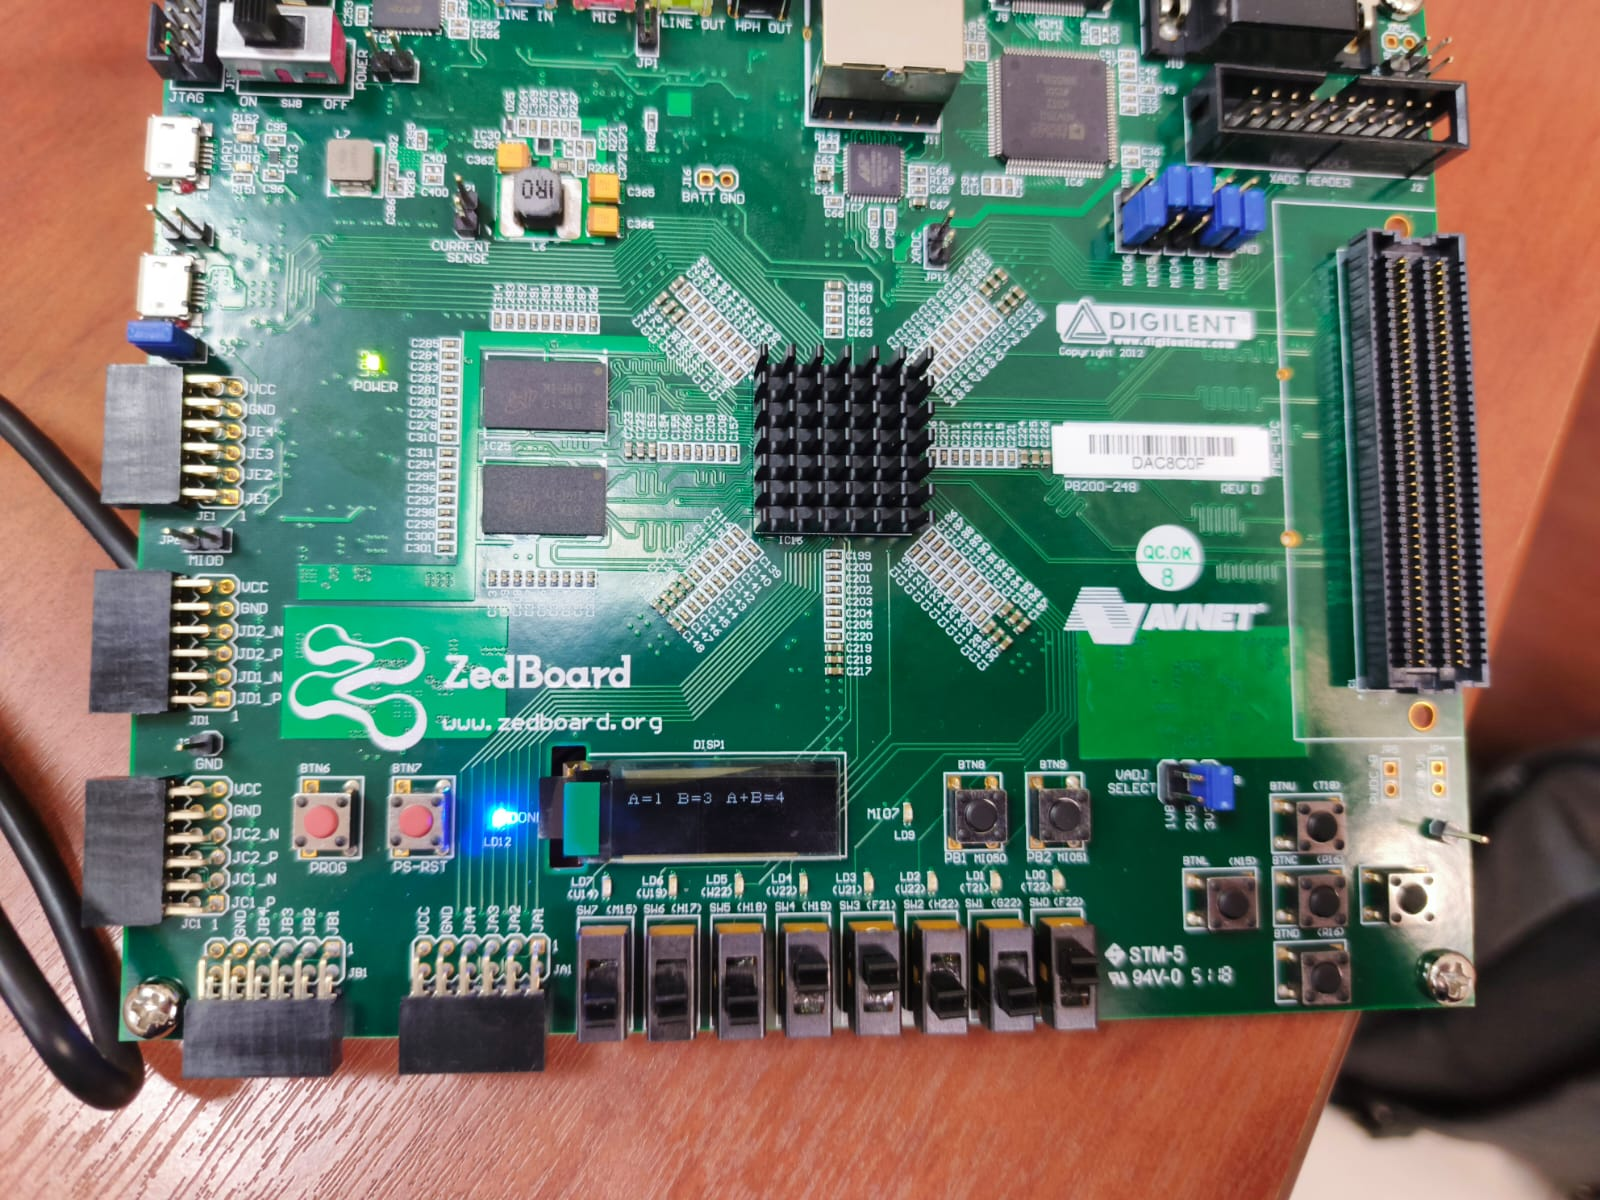
\includegraphics[width=0.78\linewidth]{result1.jpg}
    \caption{Pantalla del sumador Escenario 1.}
    \label{fig:oled-alphabet}
\end{figure}

\begin{figure}[h!]
    \centering
    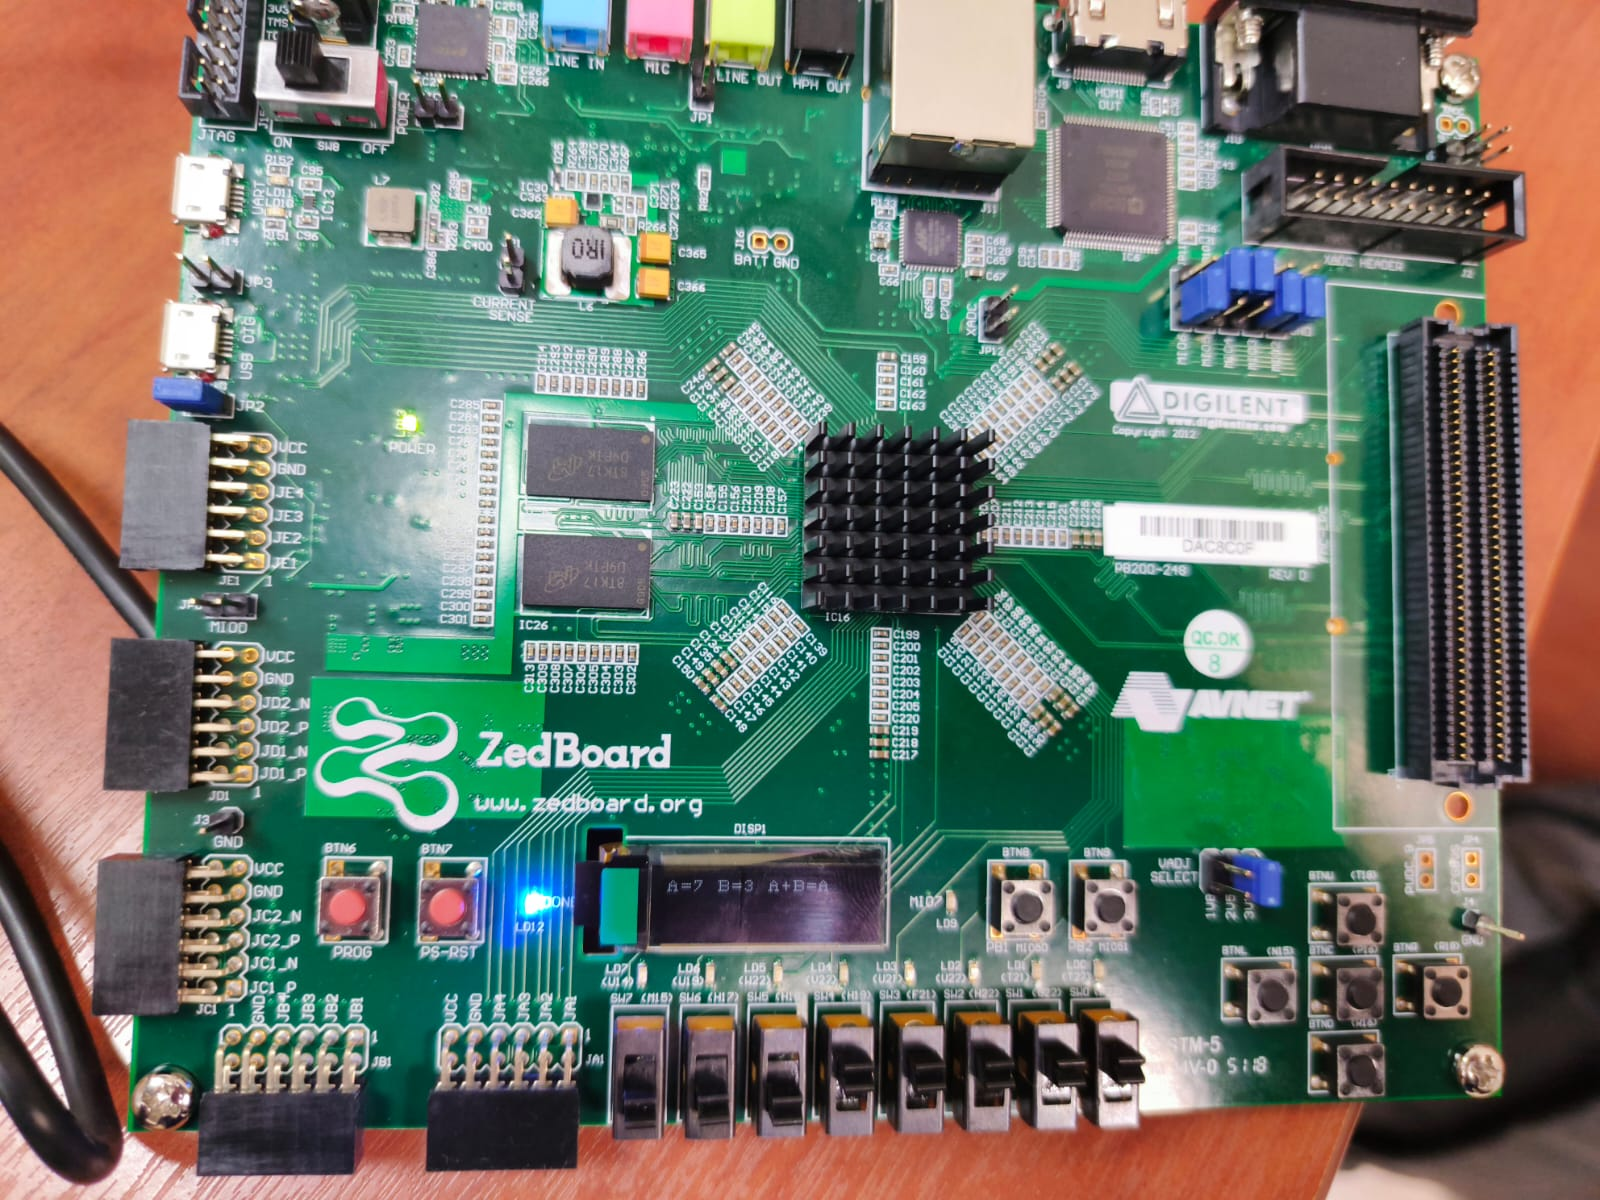
\includegraphics[width=0.78\linewidth]{result2.jpg}
    \caption{Pantalla del sumador Escenario 2.}
    \label{fig:oled-sum}
\end{figure}

\paragraph{Actualización de la visualización al cambiar \(A\) o \(B\).}
Para ver reflejado un nuevo valor de la operación en la OLED, es necesario \textbf{hacer que la FSM vuelva a construir y enviar el \emph{frame}}. En el diseño base, esto se logra \emph{cambiando de estado} (forzando un nuevo recorrido por \texttt{HelloWorldScreen} \(\rightarrow\) \texttt{UpdateScreen}). Operativamente, el flujo típico es:
\begin{enumerate}
    \item Volver a la pantalla de \emph{alfabeto} (cambio de estado).
    \item Regresar a la pantalla del \emph{sumador} (nuevo cambio de estado).
\end{enumerate}
Con ese ciclo, los caracteres se regeneran y la suma \(A{+}B\) se actualiza correctamente.




\end{document}
